\documentclass{article}
%
%	Pages: >= 4, <= 8
%
\usepackage{amsmath}%
\usepackage{amsfonts}%
\usepackage{amssymb}%
\usepackage{graphicx}
\usepackage{cite}
\usepackage{fullpage}
\usepackage{caption}
\usepackage{subcaption}
%-------------------------------------------
\begin{document}

\title{Machine Learning assignment
\\``Yeast'' data set}
\author{Tom Jaspers (105808)
\\Vrije Universiteit Brussel, Belgium}
\date{June 9, 2014}
\maketitle

\begin{abstract}
This paper examines the multi-class imbalanced classification problem of identifying location of yeast proteins using various classifiers (Decision trees, \textit{k}-Nearest Neighbor, Artificial Neural Networks). We investigate two feature selection techniques, Relief-F and Minimum Description Length Method, and show their importance by comparing the performances of the classifiers before and after applying feature selection.
\end{abstract}

\section{Introduction}

In this first section we give details about our used Yeast data set, and look at how to the deal with the class imbalance it presents. Furthermore, we present the three learning algorithms that we used to classify the data, along with the two feature selection algorithms we have applied.

The second section shows our experimental setup and the various efforts undertaken to tune the algorithms. The results from these experiments are shown in Section 3.

We conclude the paper in the fourth and final section.

\subsection{Yeast data}
The yeast data set contains 1462 rows, of which 9 are duplicates, leaving us with 1453 items. It contains 8 continuous, noisy, predictor variables (various scores based on their amino acid sequence), and 10 classes (indicating the location of the yeast protein). 

We performed a split of 75/25 to use for training, and hold out for testing, leaving us with 1090 training samples and 363 testing samples. The testing samples were held out until the day of paper writing.

From the class distribution shown in Table 1 we can conclude that the class distribution is highly skewed. Indeed, the majority of instances belong to four of the 10 classes (CYT, ME3, MIT, or NUC) making this an imbalanced problem.

\begin{table}[ht]
\centering
\begin{tabular}{cccccccccc}
  \hline
CYT & ERL & EXC & ME1 & ME2 & ME3 & MIT & NUC & POX & VAC \\  
  \hline
  438 & 5 & 35 & 43 & 51 & 162 & 244 & 425 & 20 & 30 \\
  30.14\% &  0.34\% &  2.41\% &  2.96\% &  3.51\% & 11.15\% & 16.80\% & 29.25\% &  1.38\% &  2.06\% \\ 
\end{tabular}
\end{table}

Learning from imbalanced class problems is considered to be one of the 10 challenging problems in machine learning\cite{yang200610}. The problem has been well studied in the case binary classification \cite{kotsiantis2006handling}, and is now active research topic w.r.t. multi-class imbalance\cite{wang2012multiclass}.

Strategic re-sampling is a common technique, where data is removed (undersampling) or synthetic data is generated (oversampling), for which many different methods exist \cite{chawla2011smote}.
Cost-sensitive learning has been shown to often outperform random re-sampling \cite{japkowicz2002class}. More recently, Active Learning approaches have been proposed to dealing with this problem \cite{ertekin2007learning, hospedales2013finding}.

\subsection{Learning algorithms}

\subsubsection{Decision trees}

 A decision tree is a structure where the internal nodes represent a test condition based on the value of one of the attributes, and the leaf nodes contain class values\cite{mitchell1997machine}. An instance is a assigned a label by following the nodes based on the tests until a leaf node is reached.
 
One of the most popular and commonly used implementations is C4.5\cite{quinlan1993c4}. It choses the test condition at each node using the entropy measure, such that the best attribute test allows the highest difference of entropy between the parent node and children nodes.

More recently Quilan has released a successor to C4.5, namely C5.0\footnote{C5.0: http://www.rulequest.com/see5-info.html}, incorporating several improvements, such as Adaptive Boosting. In this report, we evaluate both.


\subsubsection{Instance based learning}
In instance based learning there is no explicit generalization, but the hypotheses are constructed directly from the training instances\cite{russell13artificial}. An immediate drawback from this is that the hypothesis complexity can grow with the data size, making it more computational (and memory) intense than generalized learning algorithms.

The \textit{k}-nearest neighbors (\textit{k}-NN) is a simple, but common form of instance learning. It uses a distance metric (e.g., Euclidean) to label to an unseen case, assigning  the class most common among its \textit{k} nearest neighbors \cite{aha1991instance}. Ties are broken at random.

\subsubsection{Artificial Neural Network (ANN)}

Artificial Neural Networks are a learning model that uses multiple layers of interconnected simple units (perceptrons). It is inspired on biological learning systems that consist of large networks of neurons. ANNs are robust to errors and are often successfully applied in fields as computer vision or speech recognition\cite{mitchell1997machine}. 

We used the \textit{nnet} package provided in R, which fits a single-hidden-layer neural network, and use cross-validation to select an appropriate number of hidden units.



\subsection{Feature selection}

Dash and Liu provide a large review of feature selection techniques\cite{dash1997feature}. They categorize based on the evaluation method (e.g., distance measure, information measure, \ldots) and the generation method (random, heuristic, or complete). 
We have chosen to experimentally evaluate two of these algorithms, namely Relief-F and Minimum Description Length Method (MDLM).

\subsubsection{Relief-F}

Relief-F\cite{kononenko1994estimating} is an extension of the original Relief feature selection algorithm used in binary classification\cite{kira1992feature}. Amongst other improvements, Relief-F was made suitable for multi-class problems.

It has been shown that Relief-F is able to handle noise\cite{dash1997feature, robnik2003theoretical}, it can work continuous, discrete, and nominal data\cite{dash1997feature}, making it suited for our specific problem. We used the implementation in the \textit{FSelector} package in R.
	

\subsubsection{Minimum Description Length Method (MDLM)}

The Minimum Description Length Method (MDLM) belongs to the category of complete generative feature selection methods, using information gain as its measure\cite{sheinvald1990modeling}. It thus searches all possible subsets ($2^{8}=256$ in our case) and outputs the best one. As the name suggests, it is based on the Minimum Description Length principle, a formalization of Occam's Razor, that states that the best hypothesis for a given set is the one that leads to the best compression of the data\cite{rissanen1978modeling}.

Dash and Liu have shown that MDLM is able to handle noise, and works on continuous data\cite{dash1997feature}, making it appropriated for our problem. We used the implementation in the \textit{CORElearn} package in R\cite{procR}.

\section{Experiments}

\subsection{Performance measure}

Most algorithms are mainly compared based on their accuracy, despite it not always being representative in imbalanced problems\cite{sokolova2006beyond}. Indeed, one could trivially achieve high accuracy in an imbalanced binary classification by labeling all cases as the majority class. 
An alternative to this is plotting the receiver operating characteristics (ROC) graph. The area under the ROC curve (AUC) then provides a single scalar value between 0.5 and 1 to represent the performance, where 0.5 is as good as random, and 1.0 means no misclassification \cite{fawcett2006introduction}.

This measure is mainly used for binary classification, but has been extended for multi-class problems by n-way averaging the AUCs of one-vs-all classification \cite{hand2001simple}. The R package \textit{pROC}\cite{procR} provides an implementation for this multi-class AUC measure.  

\subsection{Decision tree}

Using the standard settings for the tree function in R we can generate a tree with 9 terminal nodes (representing 7 out of 10 class labels), and a misclassification error rate of $0.4028$. The decision tree used five out of the eight features, namely  \{alm, gvh, mcg, mit, nuc\}. Attempts to prune this tree gave no improvement, and we have thus used as is (referring to it as the \textit{simple tree} in following sections). We have shown the resulting tree in Figure 1.

\begin{figure}[htbp]
\begin{center}
  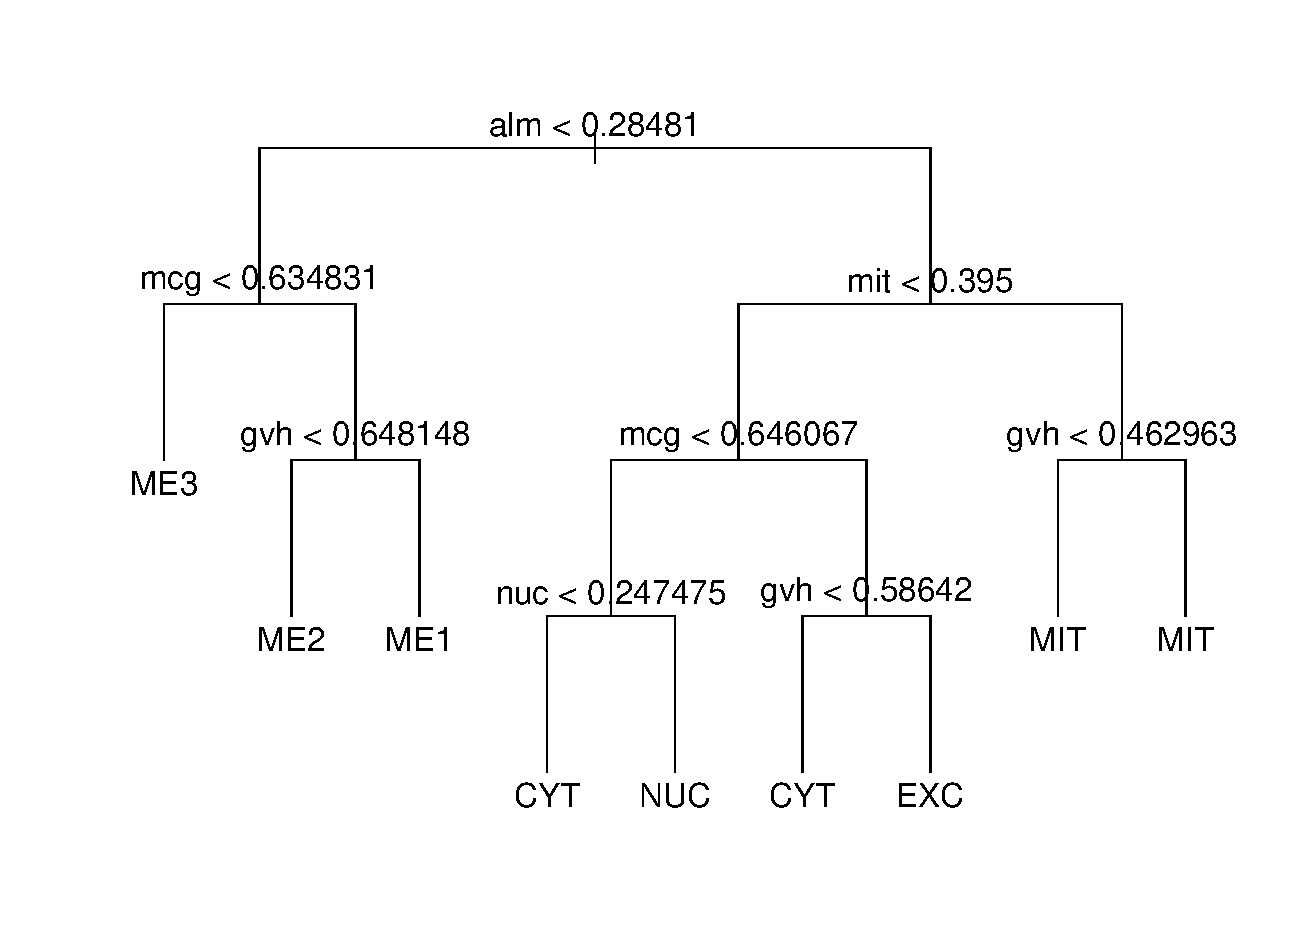
\includegraphics[width=.45\linewidth]{figures/simple-tree.pdf}
\caption{Decision tree (C4.5) obtained using the default settings. There are 9 terminal nodes that represent 7 out of 10 class labels. The features selected by the learning algorithm are  \{alm, gvh, mcg, mit, nuc\}.}
\label{default}
\end{center}
\end{figure}


Seeing as this simple tree will only be able to classify the 7 classes for which it has leaves, there is an immediate restriction as we will be unable to correctly classify 3 classes. We have thus attempted to grow a more complex tree, that allows for more overfitting. This 62-leaved tree was then pruned (using cross-validation) to one of 6 terminal nodes.

\begin{figure}[htbp]
\centering
\begin{subfigure}{.5\textwidth}
  \centering
  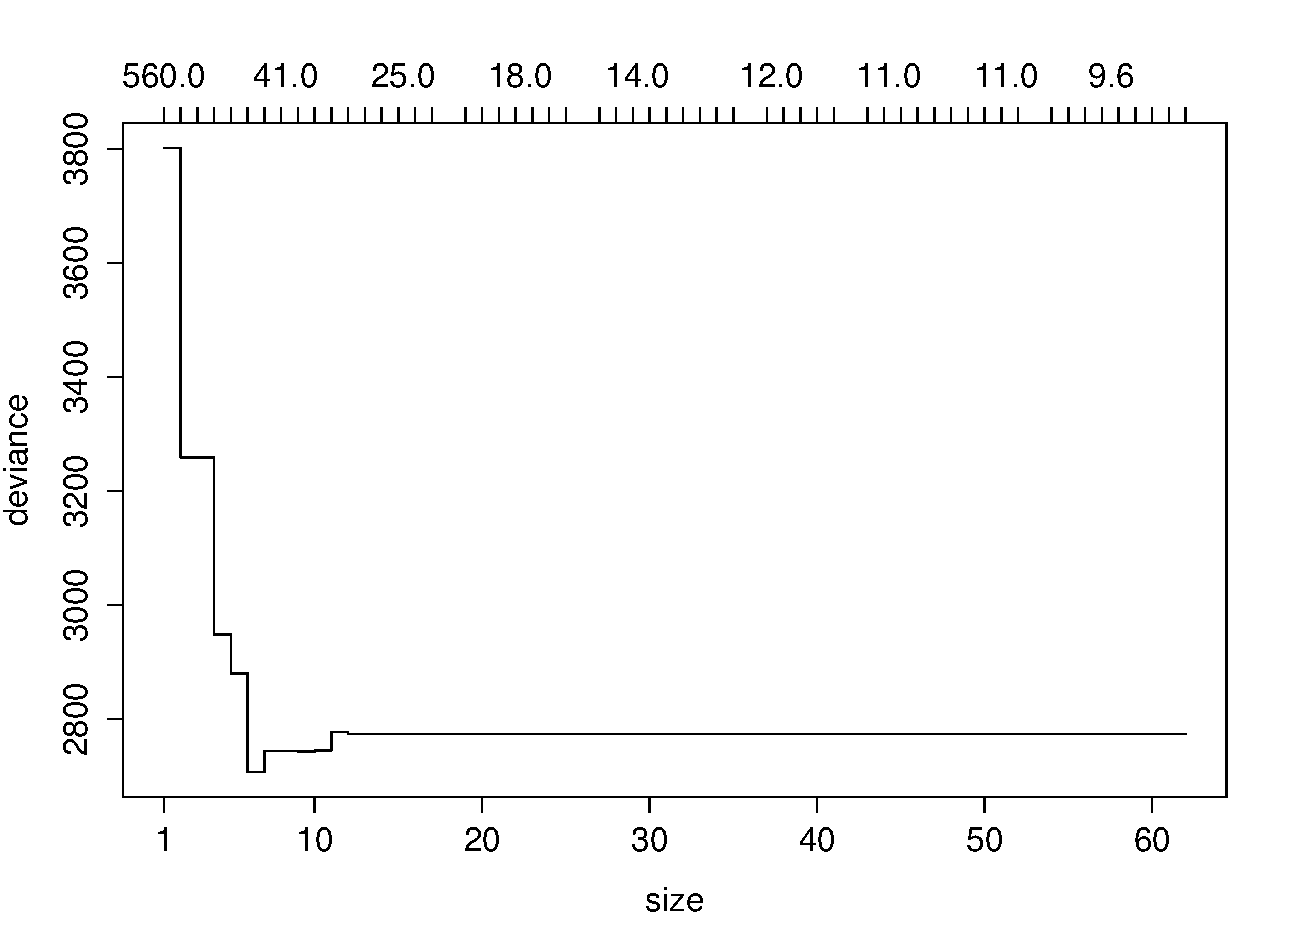
\includegraphics[width=.8\linewidth]{figures/complex-tree-cv.pdf}
  \caption{Plot of the cross-validation results}
  \label{fig:sub1}
\end{subfigure}%
\begin{subfigure}{.5\textwidth}
  \centering
  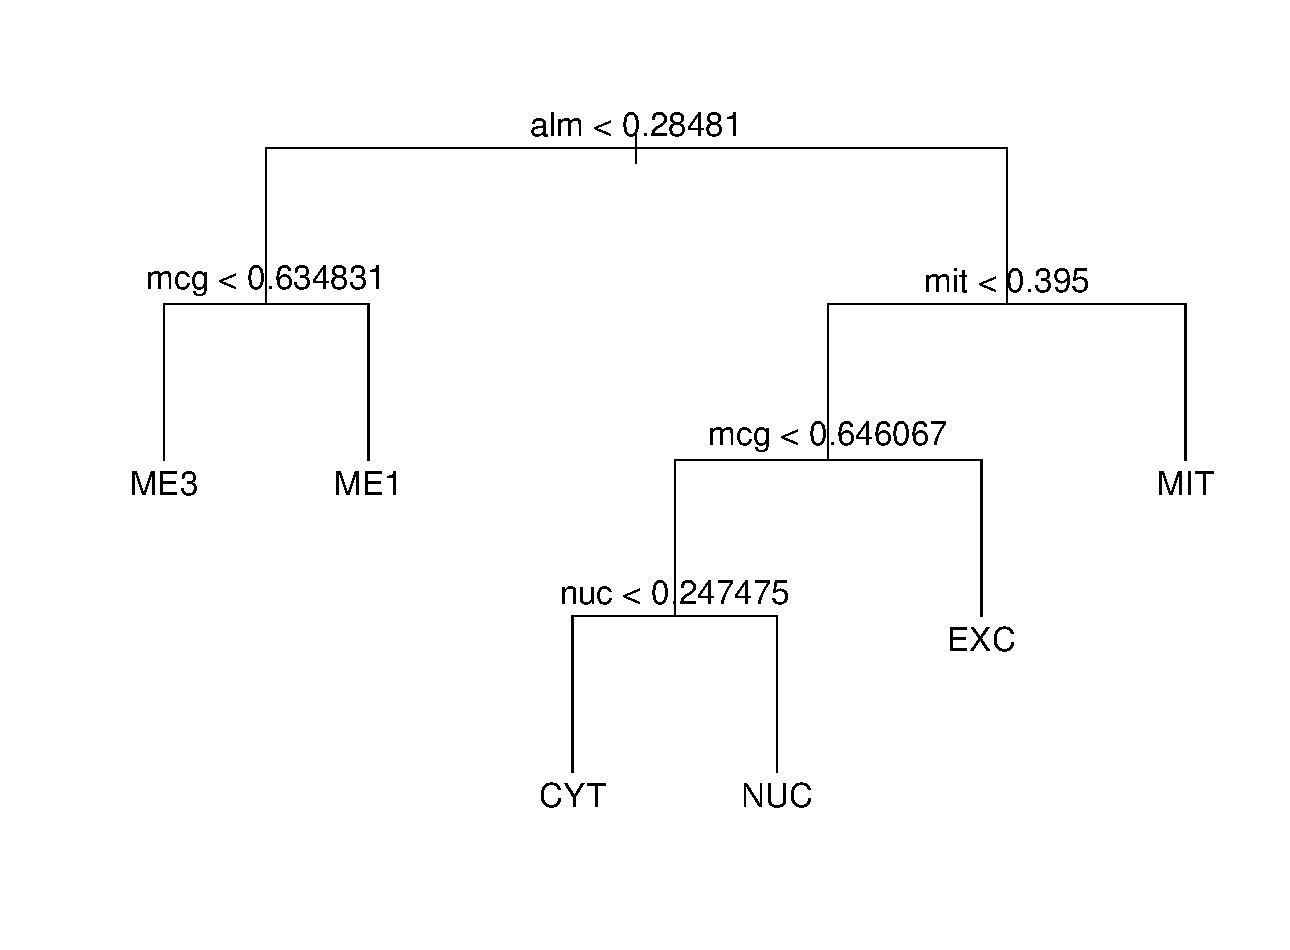
\includegraphics[width=.8\linewidth]{figures/pruned-complex-tree.pdf}
  \caption{The pruned (formerly complex) tree}
  \label{fig:sub2}
\end{subfigure}
\caption{Results from cross-validation to prune the complex tree (a), and the resulting pruned tree (b).}
\label{fig:test}
\end{figure}


We have also tested the C5.0 decision tree algorithm using the default configuration (see Results section), but no additional tuning was performed on it.





\subsection{\textit{k}-NN and ANN with full featureset}

We show the results of tuning the algorithms to find the optimal values for \textit{k} in our \textit{k}-NN algorithm, and the optimal number of units in hidden layer for ANN algorithm. We used the full featureset (all 8) for this, and present our results in the figure below.

\begin{figure}[htbp]
\centering
\begin{subfigure}{.5\textwidth}
  \centering
  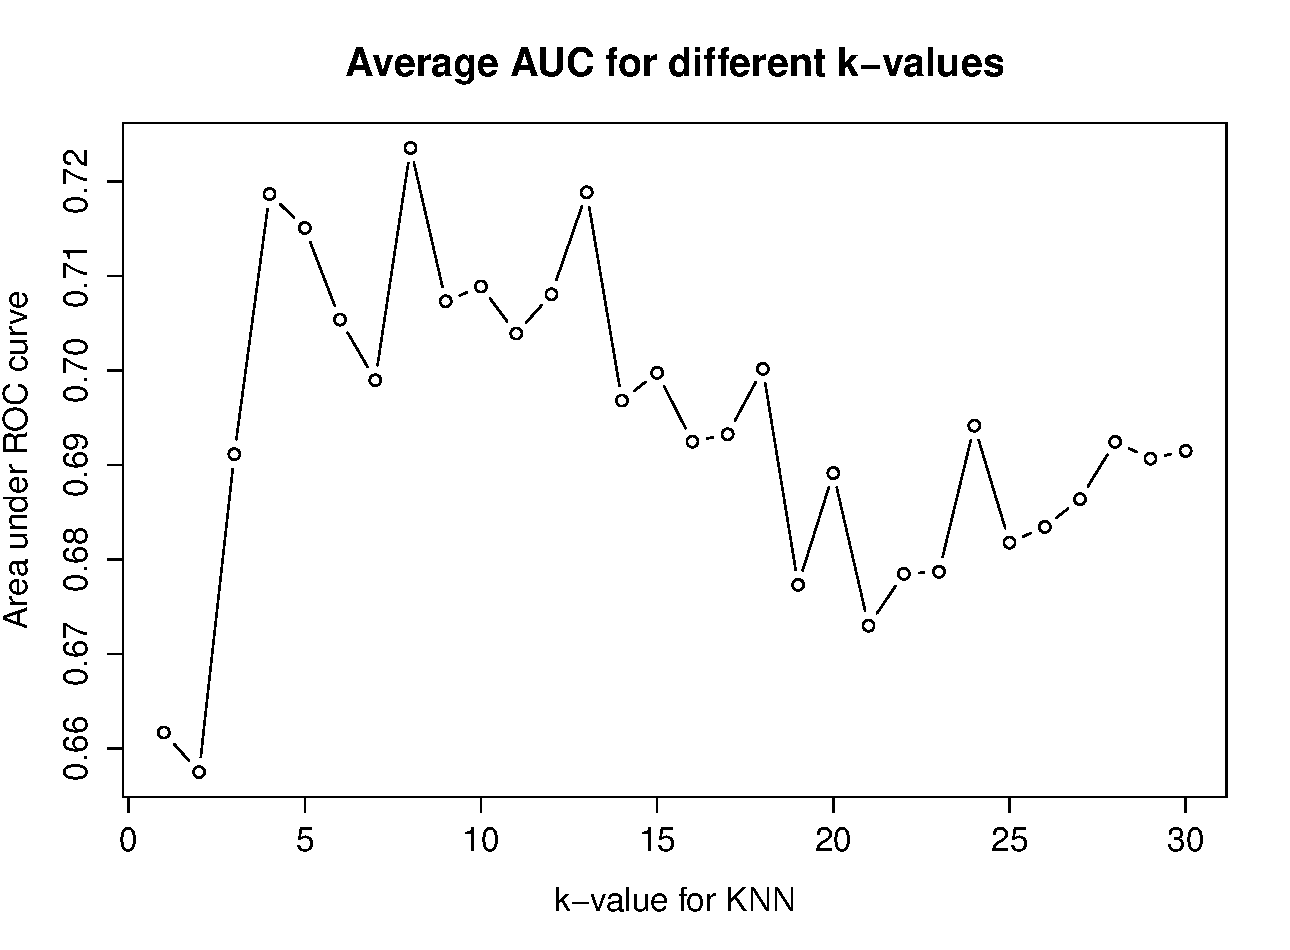
\includegraphics[width=.8\linewidth]{figures/knn-full.pdf}
  \caption{Best AUC ($0.723527$) using $k=8$}
  \label{fig:sub1}
\end{subfigure}%
\begin{subfigure}{.5\textwidth}
  \centering
  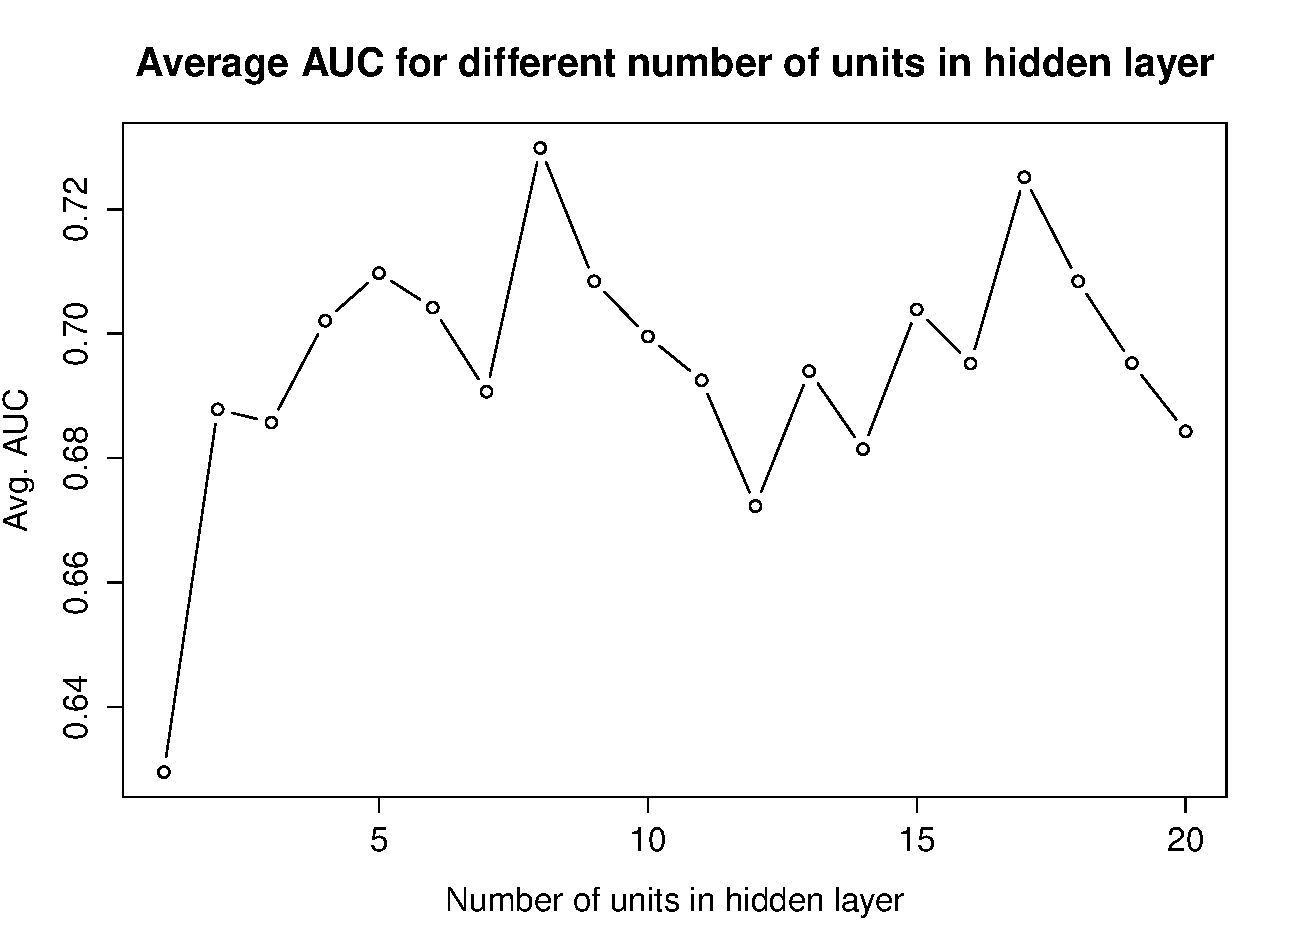
\includegraphics[width=.8\linewidth]{figures/ann-full.pdf}
  \caption{Best AUC ($0.729850$) using 8 hidden units}
  \label{fig:sub2}
\end{subfigure}
\caption{Results from 5-fold cross-validation to select the optimal value for \textit{k} in our \textit{k}-NN algorithm (a), and optimal number of units in hidden layer for ANN algorithm (b), using the full feature set.}
\label{fig:test}
\end{figure}


\subsection{\textit{k}-NN and ANN with Relief-F features}

We applied the Relief-F feature selection algorithm, and choose the five\footnote{The amount of features our decision tree ended up with.} best features provided, namely \{alm, gvh, mcg, nuc, vac\}. Four out of the five features are same as those selected by the decision tree. Instead of the \textit{mit} feature, Relief-F selected \textit{vac}.

We then re-ran cross-validation on the the \textit{k}-NN and ANN learning algorithms to find optimal values for \textit{k} and the number of hidden units, respectively.

\begin{figure}[htbp]
\centering
\begin{subfigure}{.5\textwidth}
  \centering
  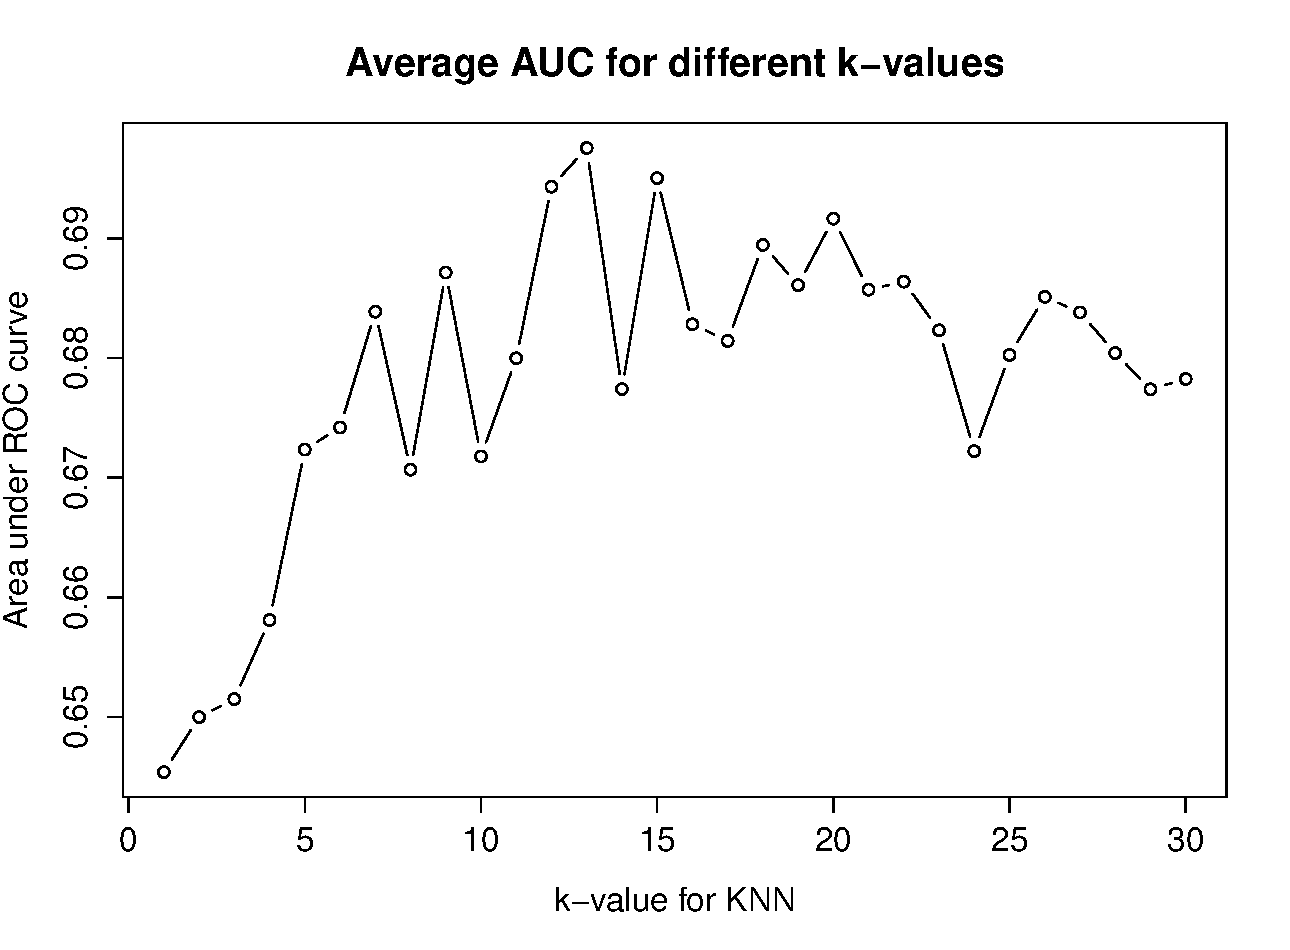
\includegraphics[width=.8\linewidth]{figures/knn-relieff.pdf}
  \caption{Best AUC ($0.6975$) using $k=13$}
  \label{fig:sub1}
\end{subfigure}%
\begin{subfigure}{.5\textwidth}
  \centering
  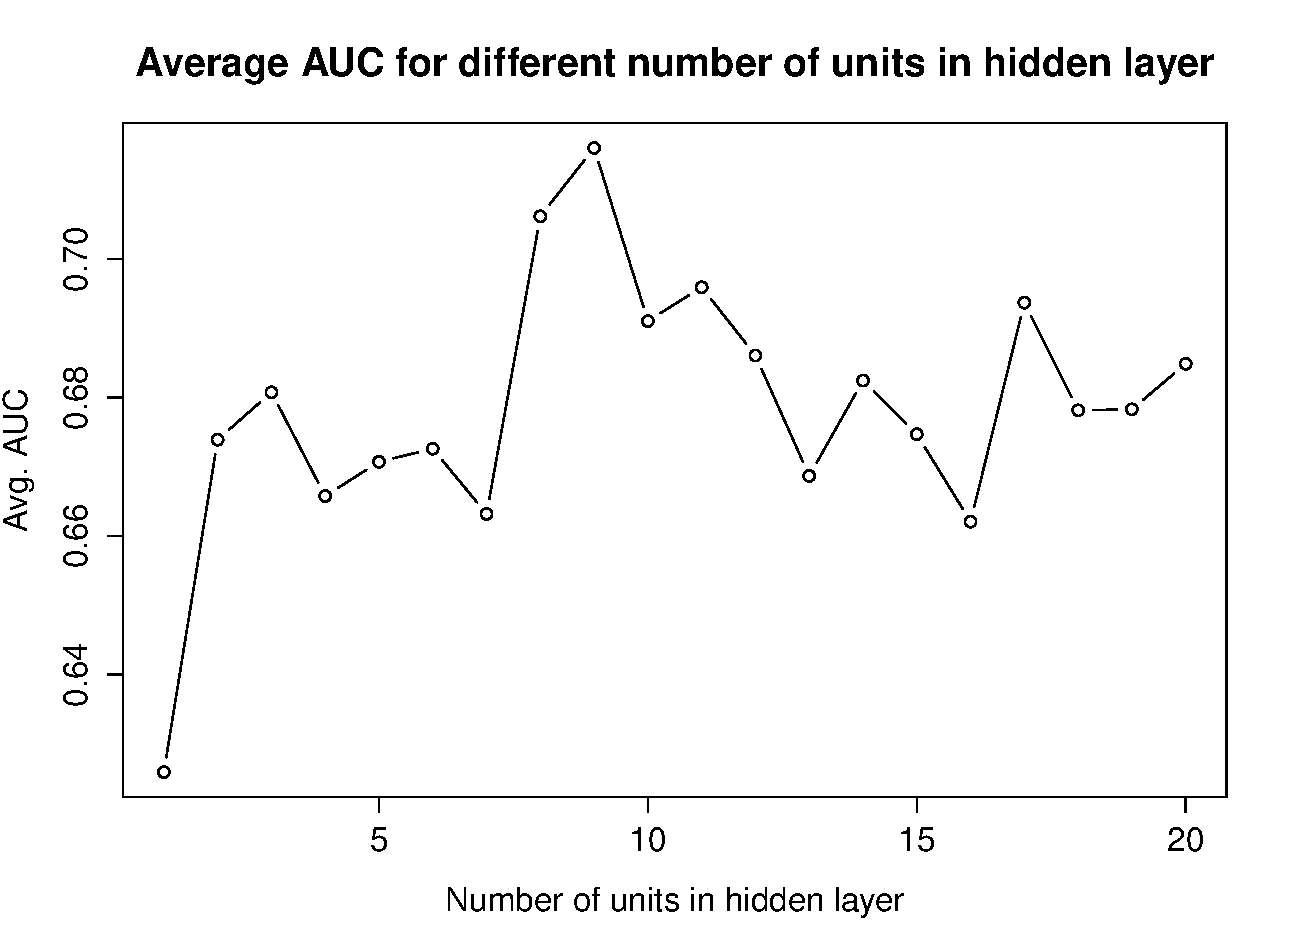
\includegraphics[width=.8\linewidth]{figures/ann-relieff.pdf}
  \caption{Best AUC ($0.7160$) using 9 hidden units}
  \label{fig:sub2}
\end{subfigure}
\caption{Results from 5-fold cross-validation to select the optimal value for \textit{k} in our \textit{k}-NN algorithm (a), and optimal number of units in hidden layer for ANN algorithm (b), using the feature set obtained through the Relief-F feature selection algorithm.}
\label{fig:test}
\end{figure}



\subsection{\textit{k}-NN and ANN with MDL features}

We applied the MDL feature selection algorithm to our dataset, and obtained the same five best features as our decision tree had obtained, namely \{alm, gvh, mcg, mit, nuc\}. The decision tree uses a form of information gain (namely difference in entropy) as a splitting criterion, which is the same kind of measure used by this MDL algorithm, and thus explains why the same set of features was obtained by both.

In order to find optimal values for \textit{k} for \textit{k}-NN and the number of hidden units for ANN, we re-ran cross-validation on these algorithms.

\begin{figure}[htbp]
\centering
\begin{subfigure}{.5\textwidth}
  \centering
  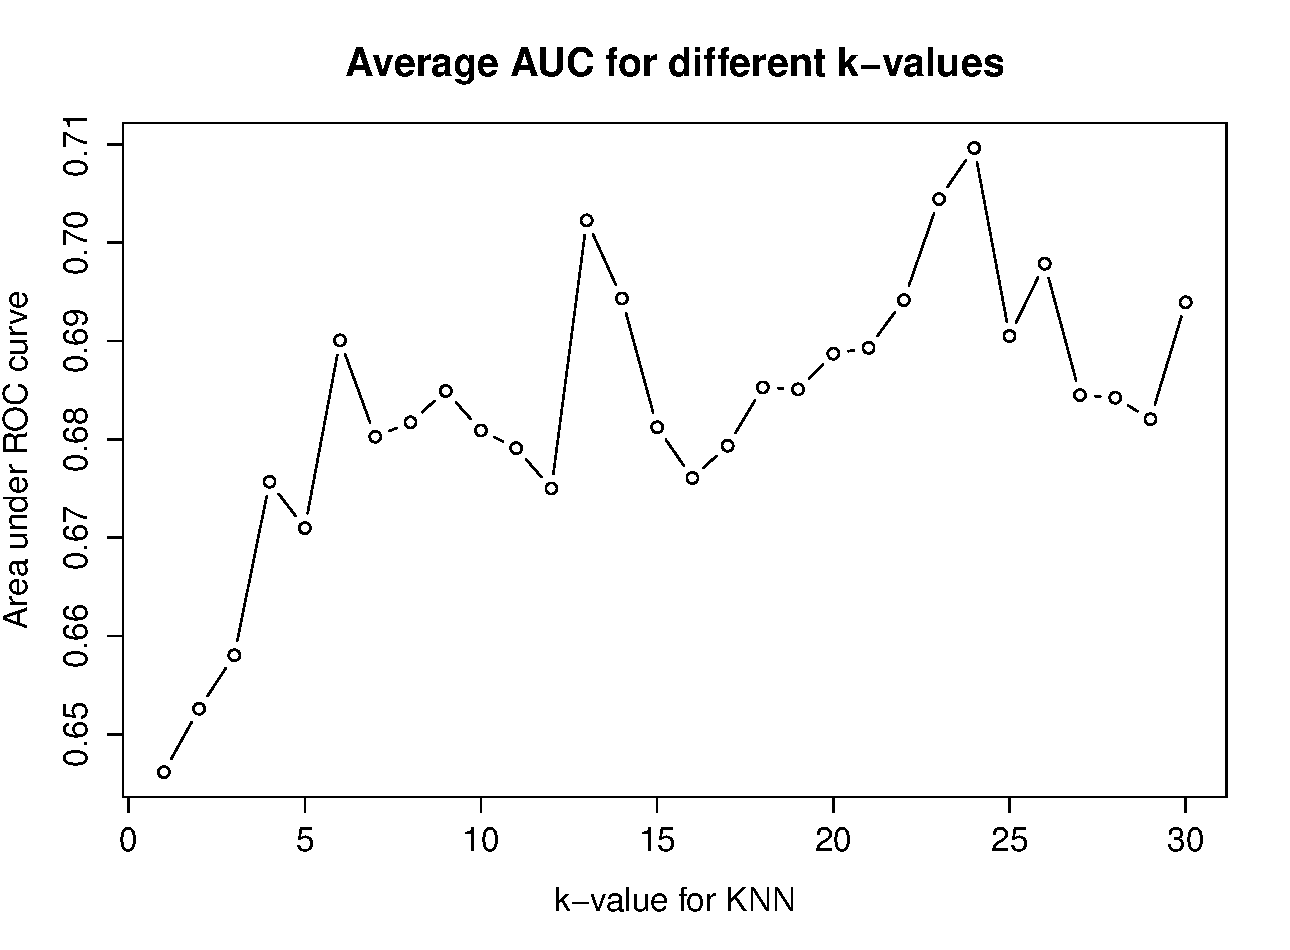
\includegraphics[width=.8\linewidth]{figures/knn-mdl.pdf}
  \caption{Best AUC ($0.7096$) using $k=24$}
  \label{fig:sub1}
\end{subfigure}%
\begin{subfigure}{.5\textwidth}
  \centering
  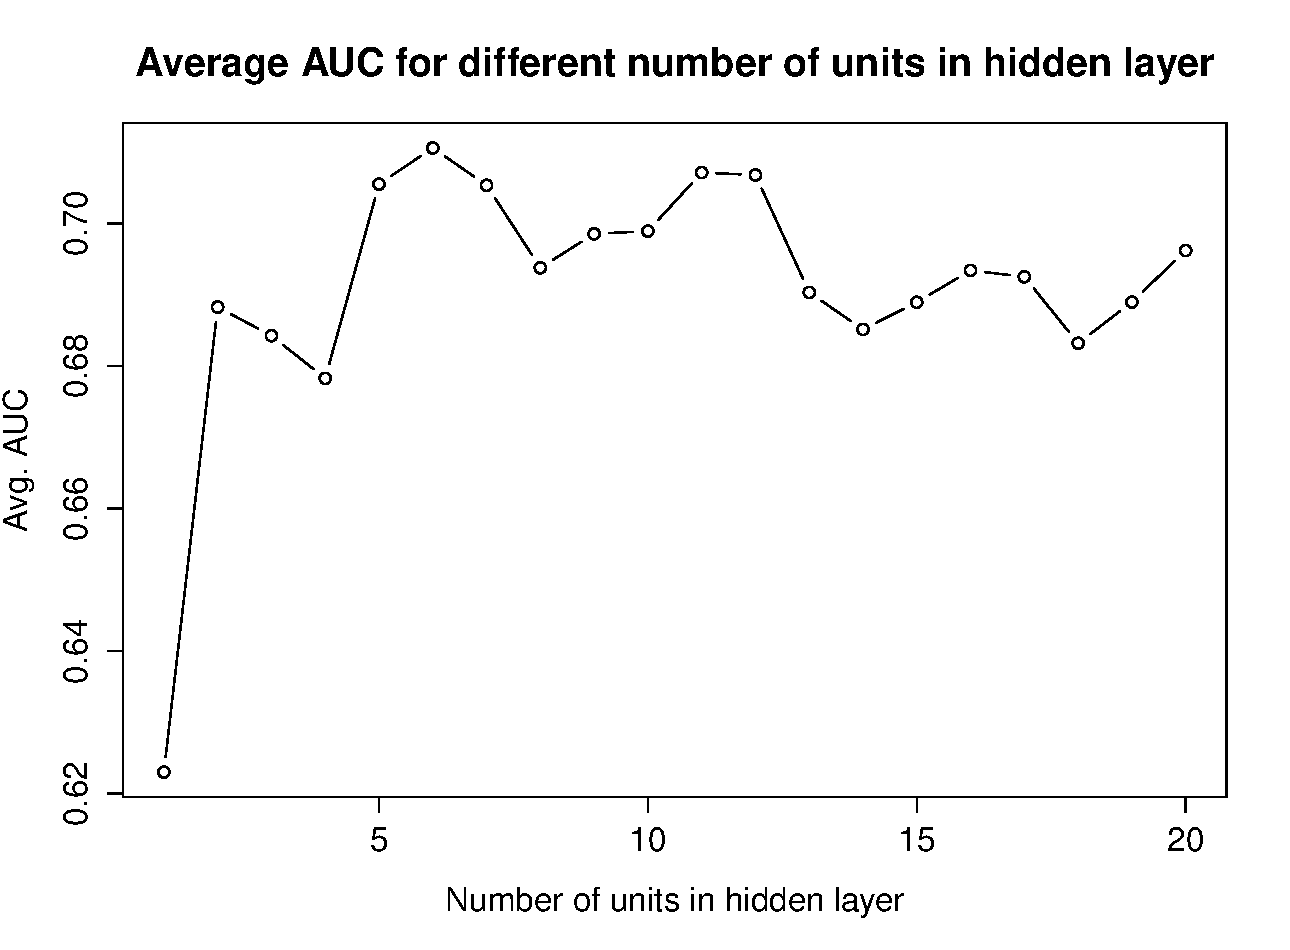
\includegraphics[width=.8\linewidth]{figures/ann-mdl.pdf}
  \caption{Best AUC ($0.7106$) using 6 hidden units}
  \label{fig:sub2}
\end{subfigure}
\caption{Results from 5-fold cross-validation to select the optimal value for \textit{k} in our \textit{k}-NN algorithm (a), and optimal number of units in hidden layer for ANN algorithm (b), using the feature set obtained through the MDML feature selection algorithm.}
\label{fig:test}
\end{figure}


\subsection{Results}

After tuning the algorithms, we trained them on the full training set of 1090 items. In the table below, we present our results from testing the trained classifiers on the independent, held-out test set of 363 items. We show the used configuration for the algorithms, and the set of features used.

\begin{table}[htbp]
\caption{Results obtained from testing the classifiers on the held-out testing set, after they were trained on the full training set.}
\begin{center}
\begin{tabular}{l l l c}
Algorithm & Configuration & Features & AUC \\
\hline  \hline
C4.5 simple & Default &  \{alm, gvh, mcg, mit, nuc\}& $0.5981$ \\
C4.5 pruned & $mincut=2$, $minsize=5$, $mindev=0.0025$ & \{alm, mcg, mit, nuc\}  & $0.6026$ \\
C5.0 & Default & All & $0.6211$ \\
\hline
 \textit{k}-NN & $k=8$ & All & $0.6710$ \\
 & $k=13$ & \{alm, gvh, mcg, nuc, vac\} & $0.5958$ \\
  & $k=24$ &\{alm, gvh, mcg, mit, nuc\} & $0.5821$ \\
 \hline
 ANN & $8$ hidden units & All & $0.6150$ \\
 & $9$ hidden units & \{alm, gvh, mcg, nuc, vac\} & $0.6366$ \\
  & $6$ hidden units & \{alm, gvh, mcg, mit, nuc\} & $0.6335$ \\
\end{tabular}
\end{center}
\label{default}
\end{table}%


The pruned, formerly more complex, C4.5 tree performs slightly better than the simple C4.5 tree. This is an interesting result, as the pruned tree only has 6 terminal nodes, compared to the 7 of the simple tree, and is thus unable to classify 4 out of 10 classes.

It is unsurprising that the C5.0 algorithm outperforms it predecessor, even with minimal tuning. Indeed, C5.0 is a much more complex model, applying boosting techniques to generate and combine multiple decision trees. 

The results of the \textit{k}-NNs are surprising in two ways. First is that it has demonstrated the best performance over all other learning algorithms, while using the full feature set. Seeing as \textit{k}-NN relies on majority voting, it is sensitive to the class imbalance, and thus we had expected worse results.
Secondly, despite being known for its sensitivity to irrelevant features, both of the feature selection algorithms have severely decreased the performance of \textit{k}-NN. We can see that the model complexity increased as well, as it used just 8 neighbors using the full featureset, but 24 using the limited featureset obtained by MDLM.

However, both Relief-F and MDLM have provided performance boosts for the ANNs. We had expected the impact of the features would be less in the ANNs.

\section{Conclusions}
We have applied three widely used learning algorithms - Decision Trees, \textit{k}-Nearest Neighbors, and Artificial Neural Networks - on the Yeast data set, a ten-class imbalanced data set with 8 predictor variables. Using the feature selection methods Relief-F and Minimum Description Length Method, we reduced the dimensionality to the same amount of features naturally used by the decision trees.  We compared the learning algorithms on the full feature set, and on the two features sets obtained after feature selection.

We found that both Relief-F and MDL provided performance boost in the neural networks. However, the \textit{k}-NN algorithm performed much worse using the limited featuresets, a surprising result considering that it is known to be sensitive to irrelevant features. The best performance was thus obtained with \textit{k}-NN ($k=8$) using the full featureset.




\bibliography{bib}{}
\bibliographystyle{plain}


\end{document}
